\documentclass[../report.tex]{subfiles}
\def\code#1{\texttt{#1}}
\begin{document}

\onehalfspacing

\newpage
\section{Hardware Design}

% TODO: Should these paragraphs be moved somewhere?

This section describes the Hardware design of Google's Verified Boot. 
Because Verified Boot is the first software run on a Chromebook, it is
responsible for initializing all of the system's hardware modules.

Verified boot main job is to check that the image being loaded originated from
Google and has not been modified. 
This is accomplished by cryptographic functions like hashing and signing.
These functions can be computationally expensive and they are used often in a
modern computer, so they are good candidate for hardware modules.  

The hardware modules can be broken into two groups, secure storage and hardware accelerator.
For secure storage there is an Flash memory module that provides non-volatile storage, and a Trusted Platform Module (TPM) that provides non-volatile storage that can be locked until the next boot.
For hardware accelerators there are the cryptographic accelerator that
implements the Secure Hash Algorithm (SHA) 

While the code for Vboot is Open Sourced and available online, the laptop's
hardware does not have source code available.
However, Google does release documents describing specifications for the
Hardware modules required. 
These specifications were used to pick Open Sourced hardware that could be made
to work with the Vboot code. 
While this means that verification was being done on different hardware, the
same techniques can easily be applied if the Chromebook hardware was ever
released.

\subsection{Flash Memory}\label{flash_mem}

The Flash Memory is an amount of extra non-volatile memory connected to every Chromebook. 
The Flash Memory contains both a Read-Only section and a Read-Write section of memory.
The Read-Only section is arguably the most important piece of hardware because it is the Root of Trust of the Vboot system.
Root of Trust means that the memory within the Read-Only section is assumed to be correct.
The code within this section is the root, or base, that is responsible for verifying the rest of the Vboot process.
The Read-Only section is assumed to be untampered because it can only be written
to by Google when the laptop was created.
The Read-Only section is enforced by a physical screw, called the Write Protect screw, which is located in the laptop.
Removing this screw removes the Root of Trust, but doing so voids the laptop's warranty.

The Read-Only memory is flashed into the laptop when the Chromebook is being built in the factory, before the Read-Only screw is added to the casing. 
The Reset Vector of the CPU points to the Read-Only flash memory, and the code located in the RO section provides information to verify the rest of the system.
In this way the RO Flash acts as the ``Root of Trust'' for the system.
In security terms, the Verified Boot process claims to be secure as long as the
Root of Trust holds (this is the claim that I will verify).

Each Chrome book comes with 8 Mbs of non-volatile Flash memory~\cite{fw-summit}.
The memory is organized according to the Flashmap which I have included in the appendix.
The Flash memory is connected to the CPU by the Serial Peripheral Interface (SPI).
The SPI driver handles the protocol and provides an interface for reading multiple bytes of of memory at once.
The Flash Memory will be the one Hardware piece needed for security that will not be emulated or verified.

\subsection{TPM}\label{sec:TPM}

The Trusted Platform Module or TPM is a general purpose cryptographic processor that is connected to a computer system for Hardware based security\cite{TPM}.
A cryptographic processor is a processor that implements a variety of
cryptographic functions, like hashing, encryption and decryption, and random
number generators. The full list of cryptographic functions can be see in
Figure~\ref{fig:tpm_hw}.
Additionally the TPM contains its own storage (volatile and non-volatile), that can be accessed from the main CPU in specific ways.
For the purpose of this report, the TPM is used as a module that can securely store keys and measurements made by the bootloader.

The physical hardware of a TPM can be created by any company, but it must conform to the standards released by the Trusted Computing Group (TCG) \cite{TCG}.
The TCG has released two specifications of TPMs and they are known as TPMs version 1.2 and 2.0.
For the scope of this project we will be looking at the TPM 1.2 specification.
The TPM specification outlines the commands, structures, and interface for the system.
The TPM commands describe the full functionality of the system by describing each command the main CPU can request.
The TPM structures describe what data structures can be passed back and forth from the CPU to the TPM, as well as what information the TPM can hold within.
The TPM interface describes the registers that are exposed to the CPU and how they should be used to send data back and forth.

\begin{figure}
  \centering
\begin{subfigure}{.4\textwidth}
  \centering
  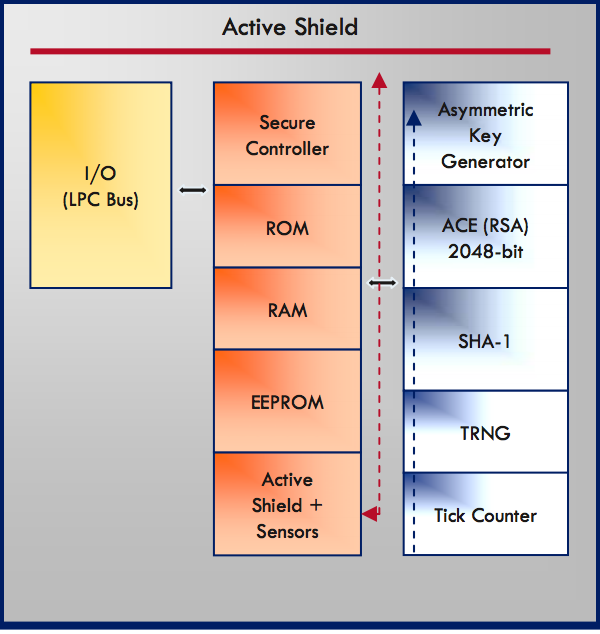
\includegraphics[width=1.0\linewidth]{tpm_hw.png}
\end{subfigure}
\begin{subfigure}{.40\textwidth}
  \centering
  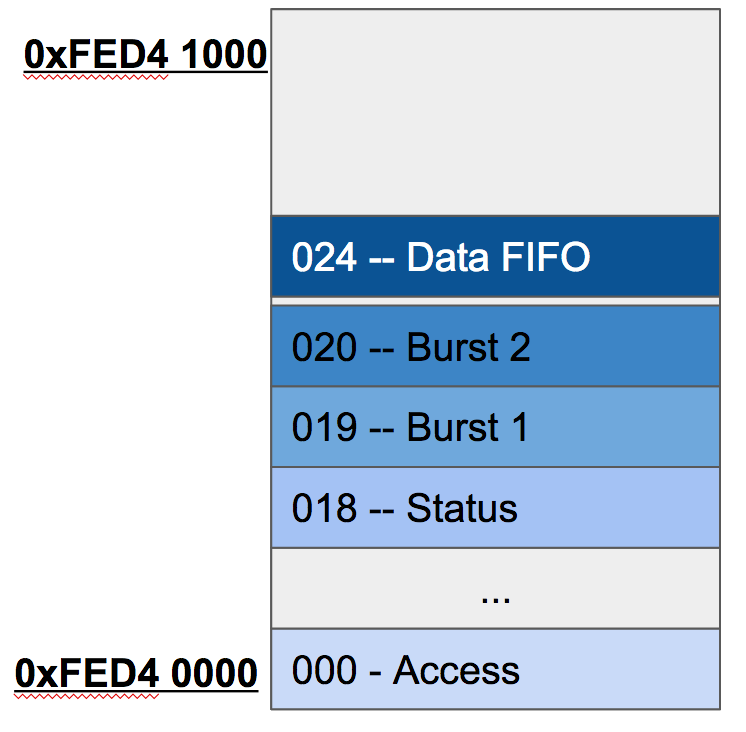
\includegraphics[width=1.0\linewidth]{tpm_regs.png}
\end{subfigure}
\caption{On the left we can see a HW block diagram of the TPM
itself\cite{tpm-slides}. 
On the right we can see the registers of the TPM that are accessed by the CPU.}
\label{fig:tpm_hw}
\end{figure}


\subsubsection{TPM Command Interface}\label{tpm_cmd_regs}

The CPU communicates to the TPM by reading and writing specific memory addresses.
These addresses allow the CPU to send multi-byte commands to the TPM and receive multi-byte responses, even though a single byte is read or written at a time.
The addresses and names of the registers can be seen in Figure~\ref{fig:tpm_hw}.
I describe the registers below.

\begin{itemize}
    \item \code{Status} --- Reading this register returns a value with flags
        that claim if the TPM is accepting a command, sending a command, or
        busy. Writing specific values to this register can tell the TPM to start
        accepting a command, or to run a command that has recently been sent.
    \item \code{Burst} --- Reading this register lets the CPU know how many
        bytes can be read (if sending a command) or written (if receiving a
        command) at a single time. This register cannot be written to.
    \item \code{Data} --- Reading this register reads one byte of data from the TPM~. Writing this register sends one byte of data to the TPM~.
\end{itemize}

% TODO: Add flow chart
% TODO: Link to code in Appendix
Sending a command serially to the TPM works in the following way.
First, the \code{Command\_Start} value is written to \code{Status}.
Second, the \code{Burst} register is read to see how many bytes the TPM can accept.
Next, the Data register is written to up to \code{Burst} times, until the command has been sent.
If the command is longer then \code{Burst} amount, \code{Burst} can be polled again until it becomes non-zero.
Finally, the \code{Command\_Go} value is written to \code{Status} and \code{Status} is polled until the TPM says that it has finished processing the command.

Receiving a command follows the process above, except that \code{Data} is read instead of written to.
Now that it is understood how commands are passed to and from the TPM, we can discuss the commands used by Google's Vboot.

\subsubsection{Platform Configuration Registers}

\begin{figure}
  \centering
  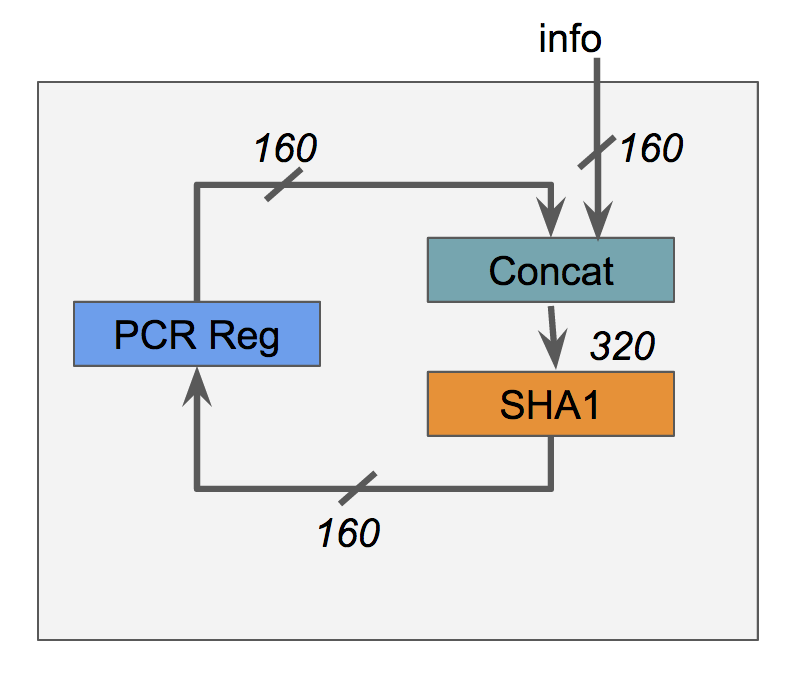
\includegraphics[width=0.4\linewidth]{pcr_alg.png}
  \caption{PCR extend Hardware Diagram}
  \label{fig:pcr_alg}
\end{figure}

One component of the TPM is called Platform Configuration Register, or PCR.
The goal of a PCR is to store measurements of the system state in a secure way. 
PCRs are secure storage because they cannot be written to directly, they are either extended or reset. 
PCRs are extended by concatenating the current the current PCR value with the input, and then storing the SHA1 hash of the result. 
Resetting the PCR changes the value to all zeros, although the PCRs used by VBoot have the reset functionality disabled.
The TCG states that only three commands affect PCRs: \code{PCR\_Extend},
\code{PCR\_Read}, and \code{PCR\_Reset}.
PCRs can also be locked, meaning that they are then unable to be extended or reset for the remainder of the system's power cycle.
The TCG specifications of these commands are included in the Appendix.


The hardware diagram of PCR\_Extend can be seen in Figure~\ref{fig:pcr_alg}.
Because the PCRs store a SHA1 Hash, they are useful for taking the measurement of a system.  
Hashing is a one way cryptographic function that is used to protect the integrity of a message.
We can think of a hash as the fingerprint of a message, because it takes an arbitrary length of data and outputs a fixed length (20 bytes).
The PCRs are iteratively extended with measurements of the system, for example,
the hash of the Read Only Firmware state, then the hash of the Read Write
Firmware state, and then the hash of the Kernel state.
The final result will be identical each time if and only if there were no changes in each of the things being measured.
By the definition of hashing, it is difficult also to find a fake configuration of the system that will hash to the same value as a correct configuration, meaning that if the hashes are equal it is reasonable to assume that the system is unchanged. 

Under specification 1.2, a TPM is required to have 21 PCRS, each PCR is 20 bytes
long and they are stored in the TPM's non-volatile storage.
Each power cycle the PCRs are reset to all 0's.

% \subsubsection{Secure Storage}
% TODO: Talk about the NV Storage Commands

\subsection{SHA}

While the TPM implements SHA hashing, Vboot also takes advantage of a dedicated
SHA hashing accelerator. 
The TPM is designed to be secure, but the SHA module is designed to be faster
than implementing the Hashing algorithm in software.
The SHA-1 hashing function can operate on any length of input.
It will iteratively hash the input in blocks of 64 bytes and output a 20 byte
hash result.

%TODO: Talk about where in opencores I found the module. 
% Talk about Bo-Yuan's ILA of the module

%TODO: Verify these registers
The SHA module is much simpler to use than the TPM in terms of Memory Mapped
Registers. 
Writing to the  \code{sha\_start} register causes the module to start the
Hashing process.
Writing to the \code{sha\_rdaddr} tells the module where to read the input data.
The module will read \code{sha\_len} bytes of the input data.
Writing to the \code{sha\_rdaddr} tells the module where to put the final 20
bytes of output data.
Reading the \code{sha\_state} register returns the state that the module is in.
This register is how a software program knows the module has completed its
operation.

\subsection{RSA}

RSA is a cryptographic platform that allows messages to be encrypted and
decrypted through the use of public and private keys.
The properties of RSA are used to send messages where the message receiver can
be sure of the identity of the message's sender. 
The structure of the RSA keys used in Vboot are outlined in
Section~\ref{sec:key_block}.

Many computer systems include RSA hardware accelerators, however Vboot does not
require one. 
The Vboot library implements all RSA algorithms in software.
These software algorithms will be used and verified instead of a hardware
module.
The possibility of adding a hardware RSA module will be discussed in the Future
Work section.

\subsection{QEMU Emulation}\label{qemu_em}

\begin{figure}
  \centering
  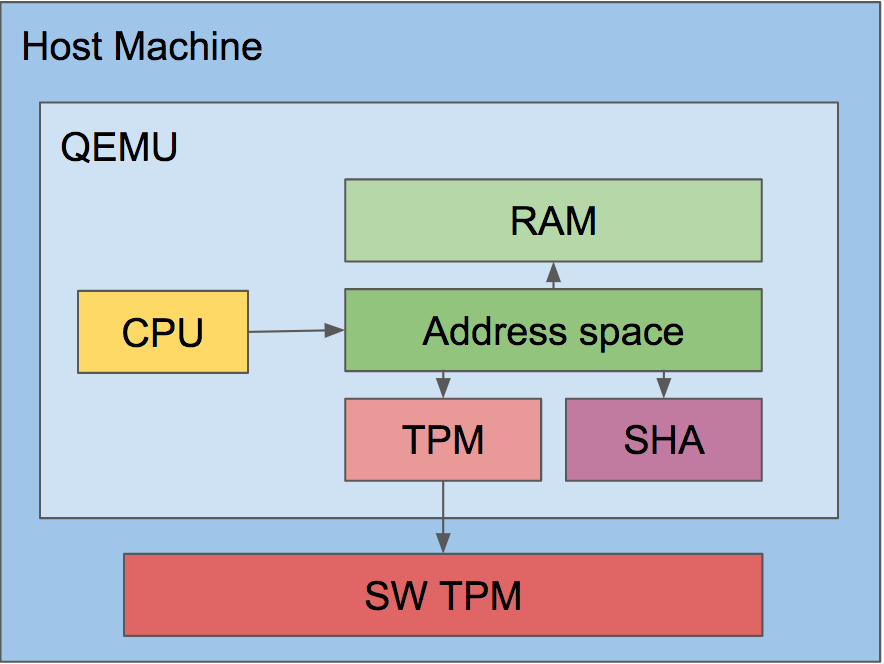
\includegraphics[width=0.4\linewidth]{qemu_layout.png}
  \caption{The QEMU layout. We can see here how the CPU and other hardware modules write RAM, and how some QEMU modules are interfaces to external software libraries.}
  \label{fig:qemu_layout}
\end{figure}

QEMU~\cite{qemu-site} is an open source emulator that is used in the report to emulate the computer running Vboot.
For this project it is used to emulate a 32 bit i386 CPU with a Memory Mapped TPM and SHA module.
To run code, I am relying on QEMU's ability to boot any image that starts with a defined multi-boot header~\cite{multiboot}.
QEMU then supplies its own bootloader, which is responsible for initializing RAM, putting the processor in 32 bit mode, and loading the image off of disk.
As we will see in Section~\ref{coreboot}, for Chromebook this job is normally taken care of by Coreboot, but for the purposes of this report it was easier to use QEMU's built-in bootloader.

The boatloader code that interacted with QEMU (included in the appendix and the github link) was based off of a project developed for Open Source at Princeton by me and Lance Goodridge.
The Open Source project allowed students to build their own Operating System from scratch and develop it within QEMU\@.
The Open Source project was repurposed by this thesis for its well-organized Makefile, linker script, and multi-boot header.
These tools allowed me to create and compile a standalone C file that could hook into the Vboot repository and run Google's Verified Boot within QEMU's virtualized Hardware.

The QEMU emulator was modified to add a TPM and a SHA module, but as mentioned in Section~\ref{flash_mem} it does not include the Flash Memory.
While the Flash Memory is important as a Root of Trust in the System, its purpose is very simple.
Its main function is to provide read-only storage, and this is not a property that is difficult to be checked.
Instead of adding Flash Memory to the QEMU emulation, I package the firmware
image with code binary using a specialized linker script. %TODO link to Linker script
The linker script loads the firmware image into the binary, and then QEMU loads
the binary into memory.
The firmware image would normally be located in the Flash Memory, but it is now
located in RAM.

% TODO: Get the SHA working
% Using my own SHA implementation, close to the one used by coreboot

\subsection{Instruction Level Abstraction (ILA)}

I am using a tool to create an Instruction Level Abstraction (ILA) of Hardware.
The ILA is used to create an abstraction of the TPM and the SHA module that can be
easily verified.
Verifying Firmware is difficult because it accesses Hardware by writing to
memory-mapped registers that trigger hardware events.
Using a software only model checker like CBMC will only see these writes
and reads to addresses, and it will not understand that a single write
corresponds to an entire Hardware operation.

\begin{figure}
  \centering
  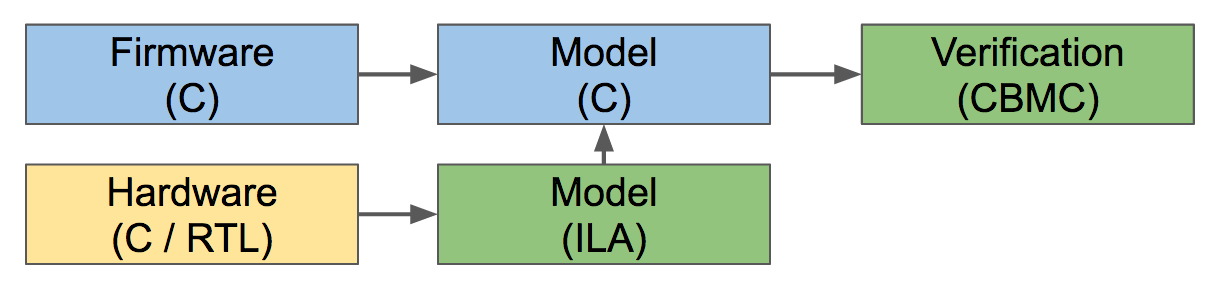
\includegraphics[width=0.6\linewidth]{ILA_flow.png}
  \caption{A flowchart of how ILA is used in the Verification process.
  In this report, ILA is used to combine the hardware model with the C program for CBMC verification.}
  \label{fig:ILA_flow}
\end{figure}

ILA provides a way to ``precisely capture updates to all firmware-accessible
states spanning cores, accelerators, and peripherals''\cite{ila-template}.
An ILA is created from either a C or Verilog program that represents the
Hardware.
To create an ILA, a programmer defines a ``template'' in python describing the
hardware.
The ILA library then verifies this template against the given C or Verilog
program to ensure that they exhibit the same behavior.
This is known as ``synthesizing'' the template into an ILA model.
The template describes each element of the hardware's state and gives a list of
how each state can be updated.
The synthesis method uses the C or Verilog program to determine when the update
functions defined by the template are activated.

The template is defined using standard update terminology for hardware, which
uses the idea of separate Decode and Execute stages.
The template's Decode stage specifies which state elements correspond to unique
instructions.
For any modules with memory mapped registers, the address of the register being
accessed, and any write information will be included in the Decode stage. 
For the TPM, the command ordinal is also included in the decode stage because
that value determines which instruction will be executed. %TODO: cite
The Execute stage involves the state update functions, and it depends on the
values in the Decode stage.
For example, the TPM ordinal determines if the TPM will execute a hashing
function or a locking function.
Actually executing the function is the purpose of the Execute stage.
The ILA synthesis is responsible for automatically mapping the Decode stage to
the Execute stage, and it uses the C or Verilog program to perform this mapping
such that the behavior of the two programs are identical.

The ILA template that is created captures the interface of the Hardware.
It produces an abstraction that is aware of how the Hardware reacts to Reads and
Writes of specific Registers.
This template can be connected back with the Firmware such that verification can
happen across the Firmware-Hardware boundary.

\end{document}
